\documentclass[11pt]{beamer}
\usetheme{Berlin}
\usepackage[utf8]{inputenc}
\usepackage[spanish]{babel}
\usepackage{amsmath}
\usepackage{amsfonts}
\usepackage{amssymb}
\usepackage{graphicx}
\usepackage{fontspec}
\setmonofont{Chomskys.otf}
\newcommand{\titulaso}[1]{{\fontspec{Chomskys.otf} #1}}

\definecolor{lightPurple}{RGB}{186, 146, 209} % Morado claro
\definecolor{darkPurple}{RGB}{98, 54, 150}    % Morado oscuro
\setbeamercolor{structure}{fg=darkPurple} % Color principal para estructuras
\setbeamercolor{frametitle}{bg=darkPurple, fg=white} % Título del marco
\setbeamercolor{block title}{bg=darkPurple, fg=white} % Título de bloques
\setbeamercolor{block body}{bg=lightPurple!30, fg=black} % Cuerpo de bloques



\author{N. Pérez-Medina}
\title{\titulaso{Modelos de regresión de series de tiempo.}}
%\setbeamercovered{transparent} 
%\setbeamertemplate{navigation symbols}{} 
\logo{
\includegraphics[scale=0.05]{logo_fing_uach_bn.png} } 
\institute{FING - UACH} 
\date{\today} 

\begin{document}

\begin{frame}
	\maketitle
\end{frame}

\begin{frame}
	\tableofcontents
\end{frame}

\section{Modelo lineal}
\begin{frame}
	\tableofcontents[currentsection] % Solo muestra la sección actual
\end{frame}

\subsection{Regresión lineal simple}
\begin{frame}{Concepto central.}
	\centering
	\hspace{-1cm}
	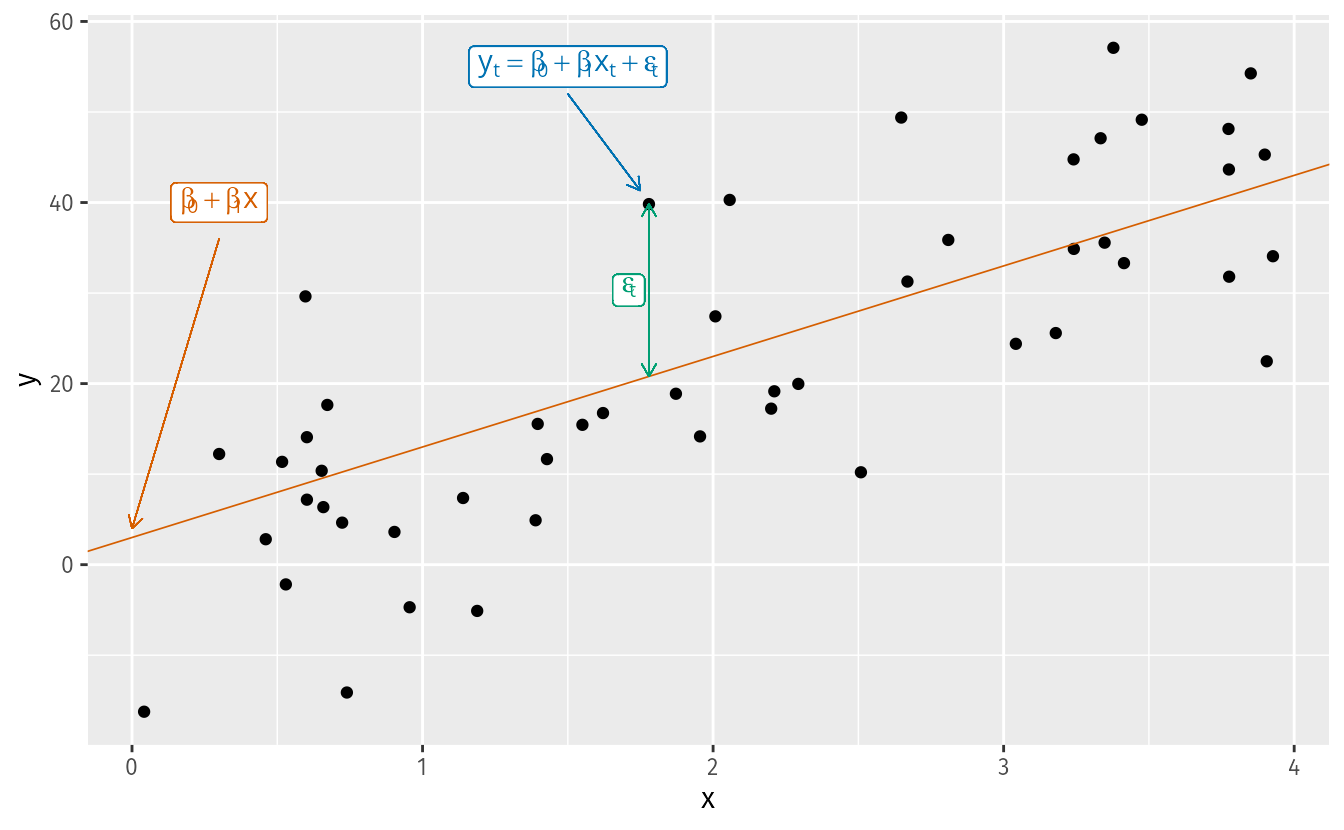
\includegraphics[scale=0.6]{fig1-introduccion.png} 
\end{frame}


\begin{frame}{Sobre los coeficientes.}
	\vspace{-0.5cm}
	\begin{block}{}
		$$ y_t = \beta_0 + \beta_1 x_t + \epsilon_t $$
	\end{block}
	\vspace{1cm}
	\begin{itemize}
		\item $\beta_0$ \textit{Valor esperado de $y$ cuando $x=0$}
		\item $\beta_1$ \textit{Cambio promedio en $y$ por cada unidad de incremento en $x$}
	\end{itemize}
\end{frame}

\begin{frame}{Ejemplo 1}
	\vspace{-1cm}
	\begin{block}{Contexto}
		Se analiza la relación entre el \textit{\textbf{gasto en consumo personal}} $y_t$ y el \textit{\textbf{ingreso disponible personal}} $x_t$ en Estados Unidos.
	\end{block}
\end{frame}

\begin{frame}{Ejemplo 1}
	\vspace{-1cm}
	\begin{block}{Contexto}
		Se analiza la relación entre el \textit{\textbf{gasto en consumo personal}} $y_t$ y el \textit{\textbf{ingreso disponible personal}} $x_t$ en Estados Unidos.
	\end{block}
	\begin{block}{Especificamente}
		 En la base de datos utilizada, las dos variables están expresadas en variaciones porcentuales trimestrales. 
		 Es decir, \textit{cada observación representa el porcentaje de cambio con respecto al trimestre anterior.}
	\end{block}
\end{frame}

\begin{frame}{Ingreso disponible personal y Gasto en consumo personal}
	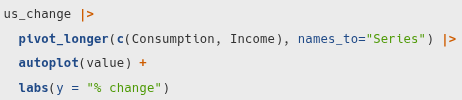
\includegraphics[scale=0.7]{EJEMPLO1-CODIGO.png} 	
\end{frame}

\begin{frame}{Ingreso disponible personal y Gasto en consumo personal}
	\hspace{-1.73cm}
	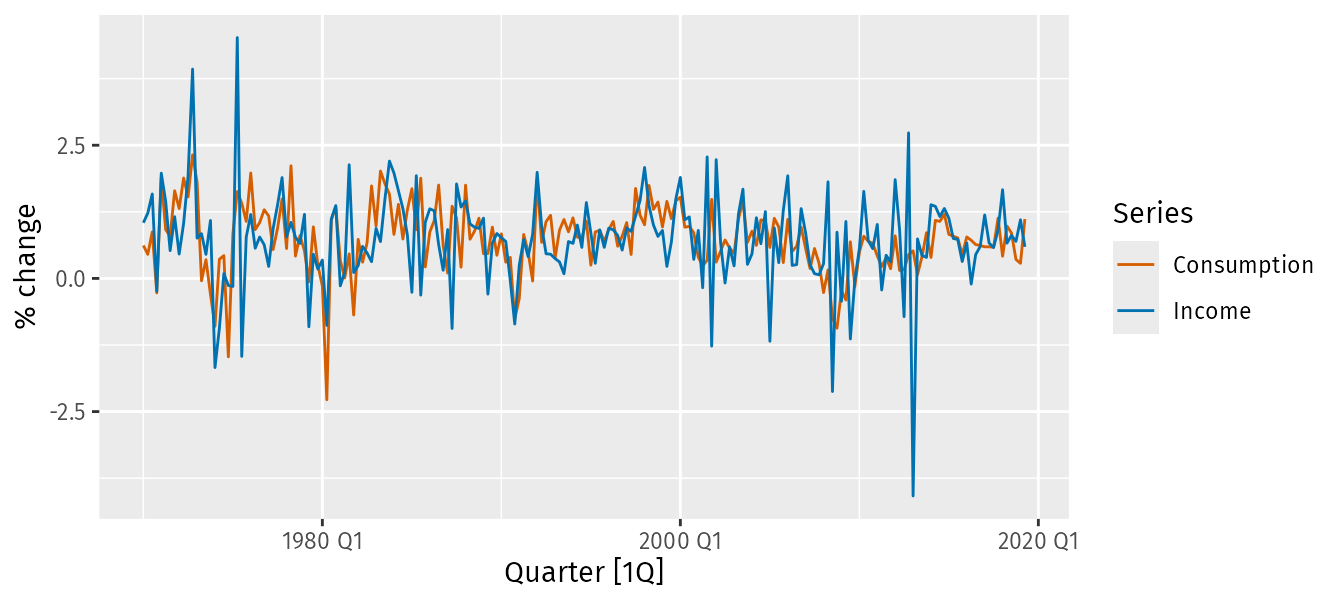
\includegraphics[scale=0.7]{ejemplo1.png} 	
\end{frame}

\begin{frame}{Diagrama de dispersión y línea ajutada}
	\centering
	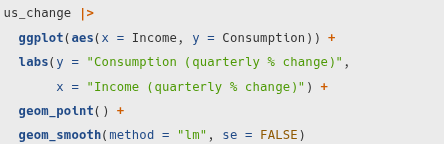
\includegraphics[scale=0.6]{EJEMPLO1-LINEA-CODIGO.png} 
\end{frame}

\begin{frame}{Diagrama de dispersión y línea ajutada}
	\centering
	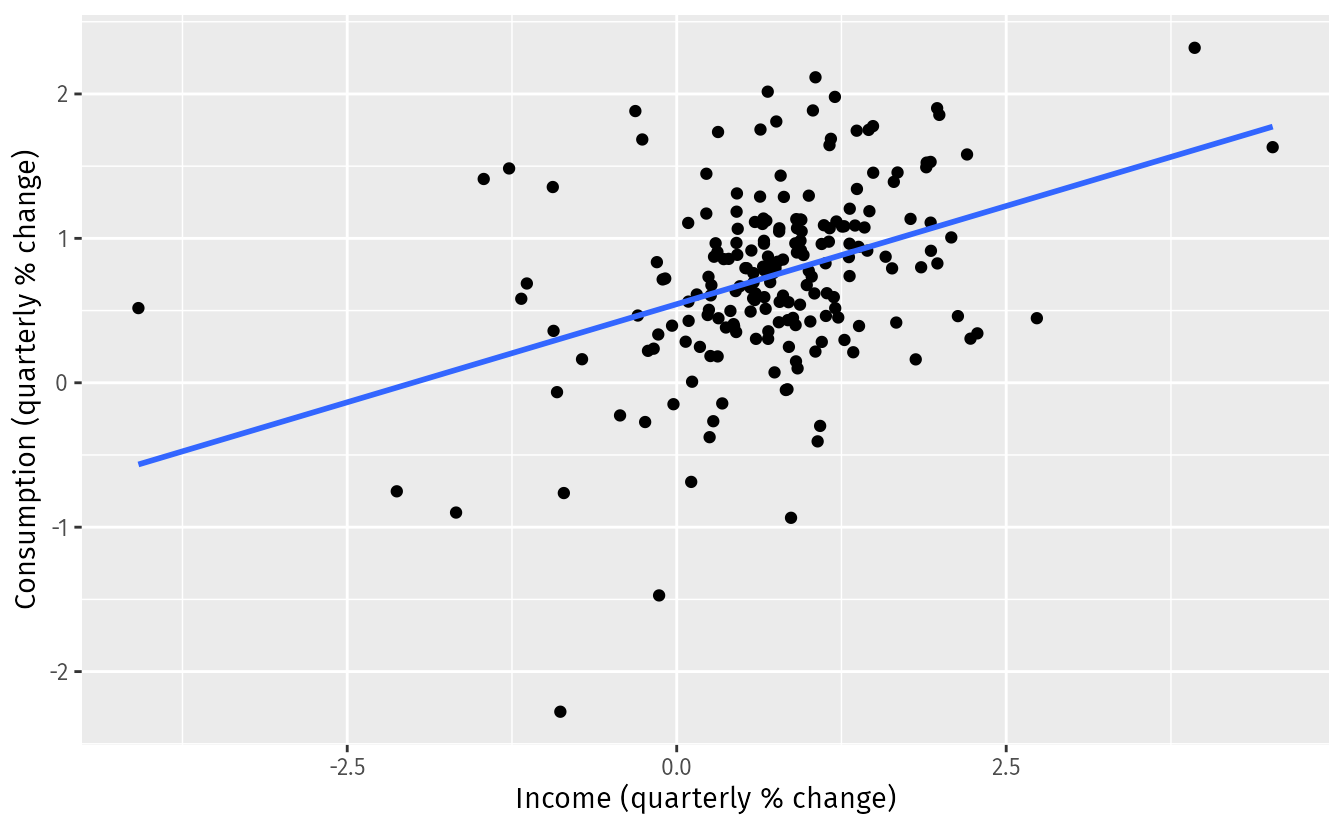
\includegraphics[scale=0.6]{ejemplo1-linea.png} 
\end{frame}

\begin{frame}{Función TSLM()}
	\centering
	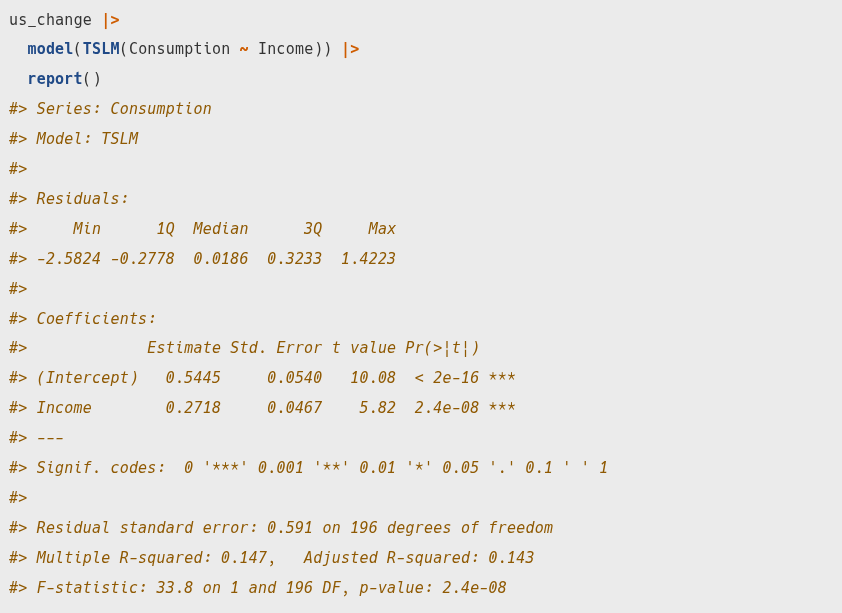
\includegraphics[scale=0.3]{codifo-tslm.png} 
\end{frame}

\begin{frame}{Modelo estimado}
	\vspace{-0.5cm}
	\begin{block}{}
		$$ y_t = 0.5445 + 0.2718 x_t + \epsilon_t $$
	\end{block}
	$\beta_0 = ​5445$ indica que, aun cuando no se observe un cambio en el \textbf{\textit{ingreso disponible personal}} $x_t$, se espera un incremento promedio del 0.59\% en el \textit{\textbf{gasto en consumo personal}} $y_t$
\end{frame}

\subsection{Regresión lineal múltiple}
\begin{frame}{Definición}
	Cuando el modelo incluye dos o más variables predictoras, se denomina \textbf{Modelo de Regresión lineal múltiple.} La forma general de este modelo es:
	\begin{block}{}
	\centering
	 $y_t = \beta_0 + \beta_1 x_{1,t} + \beta_2 x_{2,t} + \dots + \beta_k x_{k,t} + \epsilon_t$
	\end{block}
	Donde:
	\begin{itemize}
		\item $y_t$ \textit{Variable pronóstico}
		\item $x_{1,t} + x_{2,t} + \dots + x_{k,t}$ \textit{Variables predictores}
		\item $\beta_1 + \dots + \beta_k$ \textit{Coeficientes}
	\end{itemize}
\end{frame}

\begin{frame}{Ejemplo 2}
	\begin{block}{Contexto}
		Se extiende el modelo de regresión utilizado previamente para predecir el \textit{\textbf{gasto en consumo personal}} a partir de 2 variables predictoras:
		\begin{itemize}
			\item \textit{Income: }variación porcentual del ingreso disponible personal.
			\item \textit{Savings:} variación porcentual en el ahorro.
			
			\item \textit{Unemployment:} cambio trimestral en la tasa de desempleo.
		\end{itemize}
	\end{block}
\end{frame}

\begin{frame}{Producción industrial, ahorro personal y tasa de desempleo en EE. UU}
	\centering
	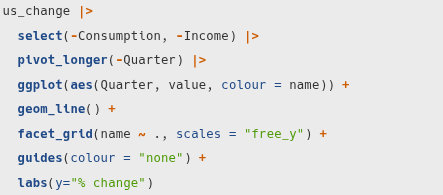
\includegraphics[scale=0.6]{ejemplo2-codigo.png} 

\end{frame}

\begin{frame}{Producción industrial, ahorro personal y tasa de desempleo en EE. UU}
	\centering
	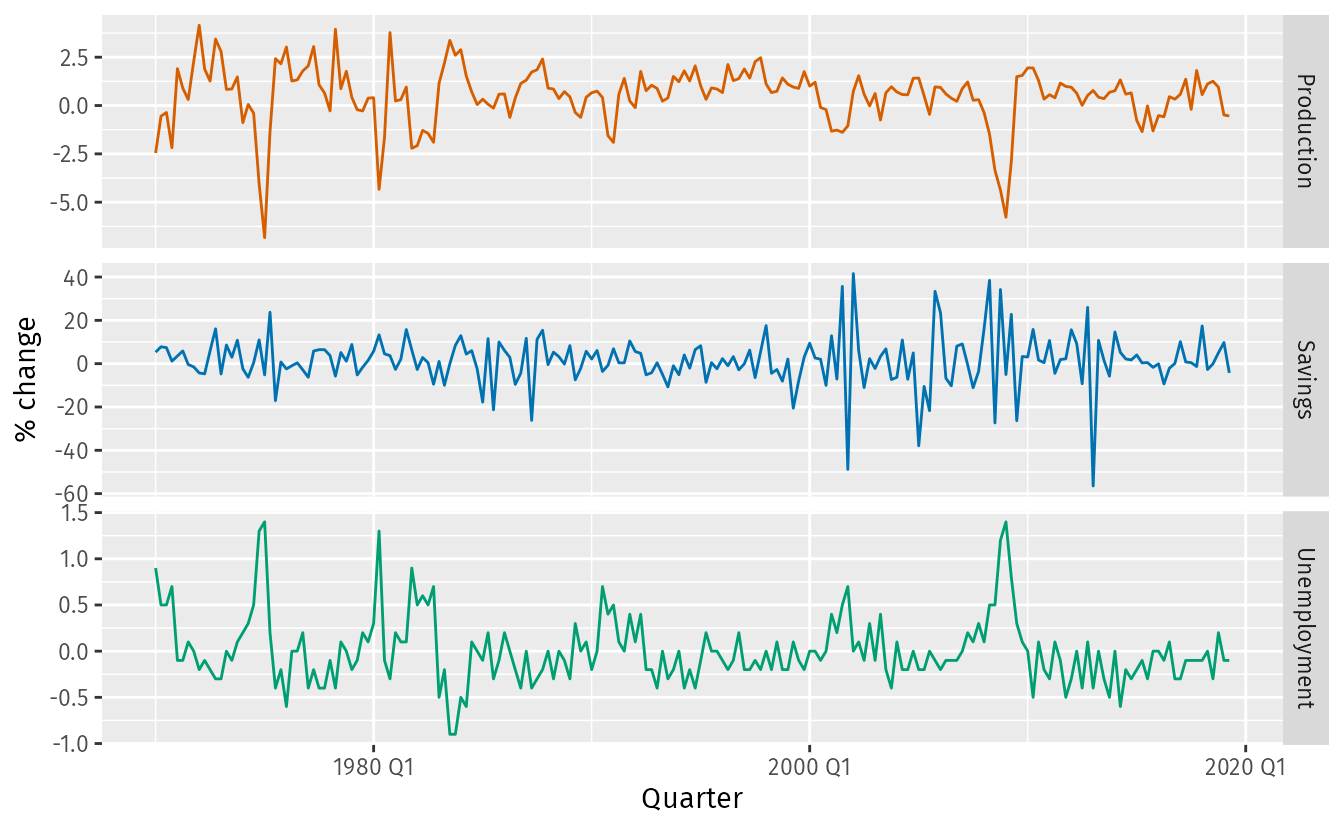
\includegraphics[scale=0.6]{ejemplo2.png} 

\end{frame}

\begin{frame}{Matriz de gráficos de dispersión}
	\centering
	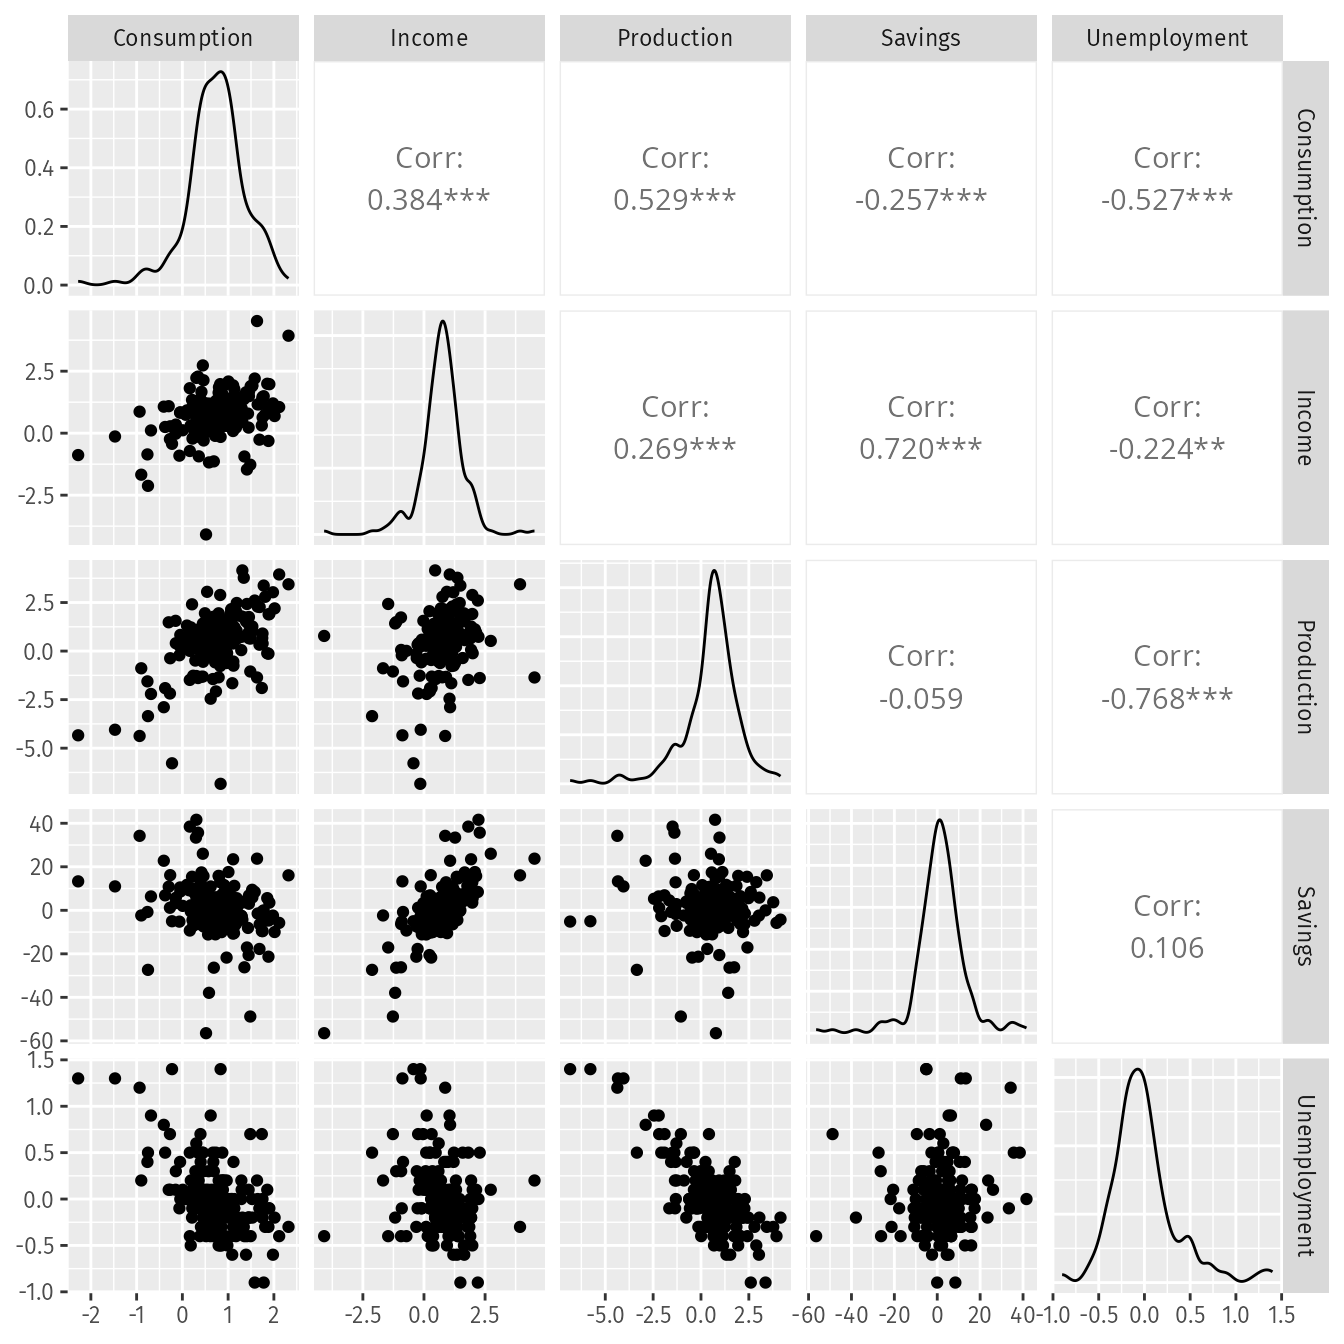
\includegraphics[scale=0.35]{ScatterMatrix-1.png} 
\end{frame}

\subsection{Supuestos}
\begin{frame}{¿Qué se supone que suponemos?}
	\begin{block}{}
		\begin{enumerate}
			\item Supuesto general del modelo
			\item Supuestos sobre los errores
			\item Supuesto sobre las variables predictores
		\end{enumerate}
	\end{block}
\end{frame}

\begin{frame}{1- Supuesto general del modelo}
	\begin{block}{}
		Se \textit{asume} que la relación entre la \textbf{\textbf{variable de pronóstico}} y las \textbf{\textit{variables predictoras}} puede aproximarse mediante una \textbf{relación lineal.}
	\end{block}
\end{frame}

\begin{frame}{2- Supuestos sobre los errores}
	\begin{block}{}
		\begin{itemize}
			\item \textbf{Media cero:} 
			\item \textbf{No autocorrelación:} 
			\item \textbf{Independencia respecto a los predictores:} 
		\end{itemize}
	\end{block}
\end{frame}

\begin{frame}{2- Supuestos sobre los errores}
	\begin{block}{}
		\begin{itemize}
			\item \textbf{Media cero:} De lo contrario, los pronósticos estarán sesgados.
			\item \textbf{No autocorrelación:} Si hay autocorrelación, se pierde eficiencia en el pronóstico, ya que hay información no aprovechada.
			\item \textbf{Independencia respecto a los predictores:} Si los errores están correlacionados con las variables predictoras, se viola la suposición de que toda la información sistemática está en el modelo.
		\end{itemize}
	\end{block}
\end{frame}

\begin{frame}{3- Supuesto sobre las variables predictoras}
	\begin{block}{}
		\begin{itemize}
			\item Las variables $x$ se tratan como \textbf{no aleatorias.} 
		\end{itemize}
	\end{block}
\end{frame}

\section{Estimación de mínimos cuadrados}
\begin{frame}
	\tableofcontents[currentsection] % Solo muestra la sección actual
\end{frame}
\subsection{Principio}
\begin{frame}{Principio de los Mínimos Cuadrados}
	\begin{block}{}
	\centering
	 $y_t = \beta_0 + \beta_1 x_{1,t} + \beta_2 x_{2,t} + \dots + \beta_k x_{k,t} + \epsilon_t$
	\end{block}

\end{frame}

\begin{frame}{Principio de los Mínimos Cuadrados}
	\begin{block}{}
	\centering
	 $\epsilon_t = y_t-(\beta_0 + \beta_1 x_{1,t} + \beta_2 x_{2,t} + \dots + \beta_k x_{k,t} )$
	\end{block}

\end{frame}

\begin{frame}{Principio de los Mínimos Cuadrados}
	\begin{block}{}
	\centering
	 $\epsilon_t^2 = (y_t-(\beta_0 + \beta_1 x_{1,t} + \beta_2 x_{2,t} + \dots + \beta_k x_{k,t} ))^2$
	\end{block}

\end{frame}

\begin{frame}{Principio de los Mínimos Cuadrados}
	\begin{block}{}
	\centering
	 $\sum_{t=1}^{T} \epsilon_t^2 = \sum_{t=1}^{T} (y_t-(\beta_0 + \beta_1 x_{1,t} + \beta_2 x_{2,t} + \dots + \beta_k x_{k,t} ))^2$
	\end{block}
	
\end{frame}

\begin{frame}{Principio de los Mínimos Cuadrados}
	\begin{block}{}
	\centering
	 $\sum_{t=1}^{T} \epsilon_t^2 = \sum_{t=1}^{T} (y_t-(\beta_0 + \beta_1 x_{1,t} + \beta_2 x_{2,t} + \dots + \beta_k x_{k,t} ))^2$
	\end{block}
	
	El proceso de encontrar \textbf{los mejores estimadores de los coeficientes} se conoce como \textit{ajustar el modelo a los datos} o \textit{entrenar el modelo}.

\end{frame}

\subsection{Estimación por TSLM}
\begin{frame}{Mínimos cuadrados con función TSLM}
	\centering
	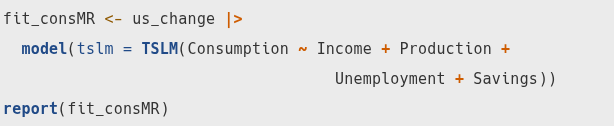
\includegraphics[scale=0.5]{tslm-rlm-codigo.png} 
\end{frame}

\begin{frame}{Mínimos cuadrados con función TSLM}
	\centering
	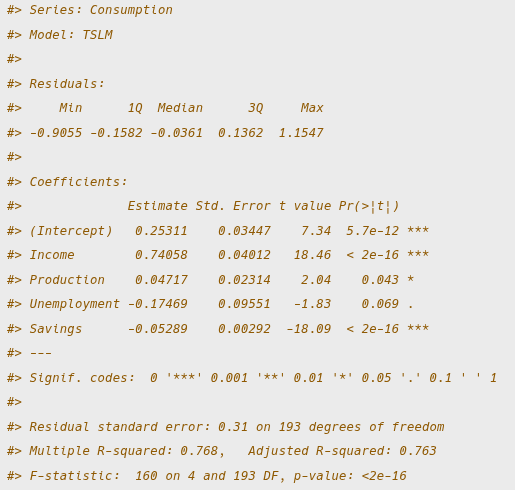
\includegraphics[scale=0.4]{tslm-rlm-respuesta.png} 
\end{frame}

\begin{frame}{Valor-t y Valor-p}
	\begin{block}{\textbf{Valor t}}
		Mide cuán grande es el coeficiente estimado en relación con su error estándar.
	\end{block}
	\begin{block}{\textbf{Valor p}}
		 Indica la probabilidad de que el coeficiente observado se haya producido por azar.
	\end{block}
	Aunque \textit{útiles} para \textbf{entender la relevancia de los predictores}, estos valores no son \textit{cruciales} para la predicción futura de los datos.
\end{frame}

\subsection{Valores ajustados}
\begin{frame}{¿Qué hacemos con lo que obtenemos?}
	\begin{block}{}
		Las predicciones\footnote{No son pronósticos genuinos, son las predicciones para los mismos datos que se usaron para ajustar el modelo.} de $y$ pueden obtenerse utilizando los \textbf{coeficientes estimados} en la ecuación de regresión y poniendo el término de error a cero.
		$$ \hat{y_t}  = \hat{\beta_0} + \hat{\beta_1} x_{1,t} + \hat{\beta_2} x_{2,t} + \dots + \hat{\beta_k} x_{k,t} $$
	\end{block}
\end{frame}

\begin{frame}{Valores ajustados y Valores reales}
	\centering
	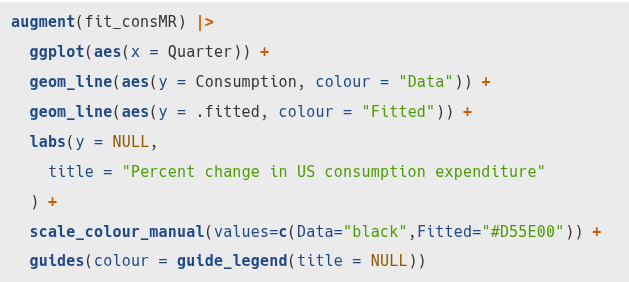
\includegraphics[scale=0.5]{modelo-ajustado-codigo.png} 
\end{frame}

\begin{frame}{Valores ajustados y Valores reales}
	\centering
	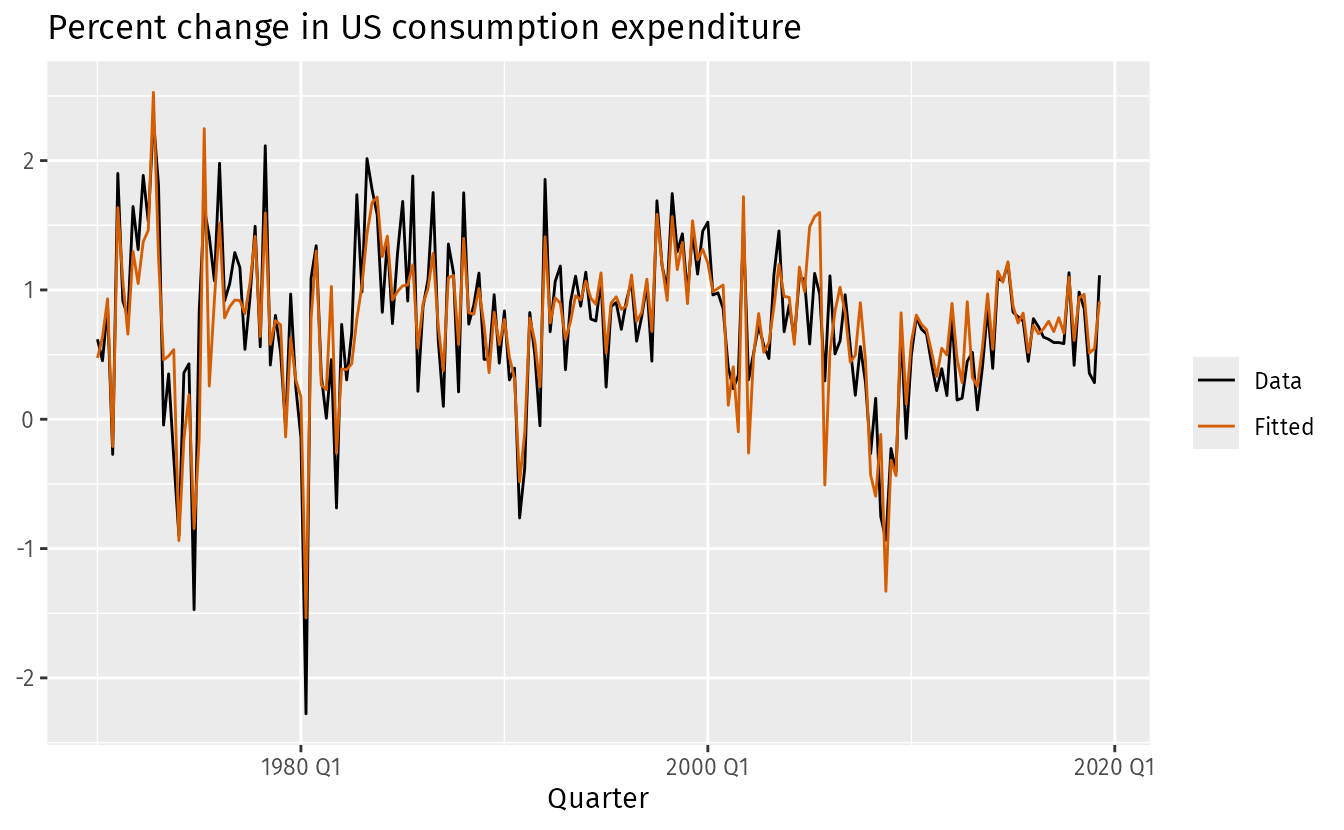
\includegraphics[scale=0.6]{modelo-ajustado-vs-real.png} 
\end{frame}

\begin{frame}{Valores ajustados vs. Valores reales}
	\centering
	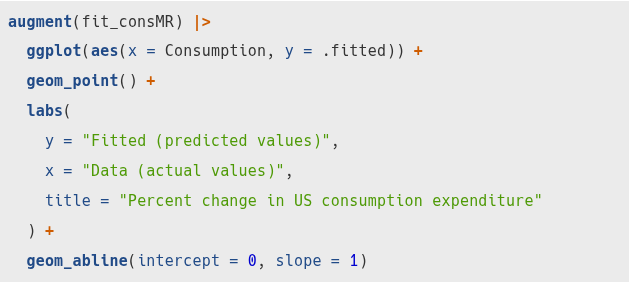
\includegraphics[scale=0.5]{ajustado-vs-real-codigo.png} 
\end{frame}

\begin{frame}{Valores ajustados vs. Valores reales}
	\centering
	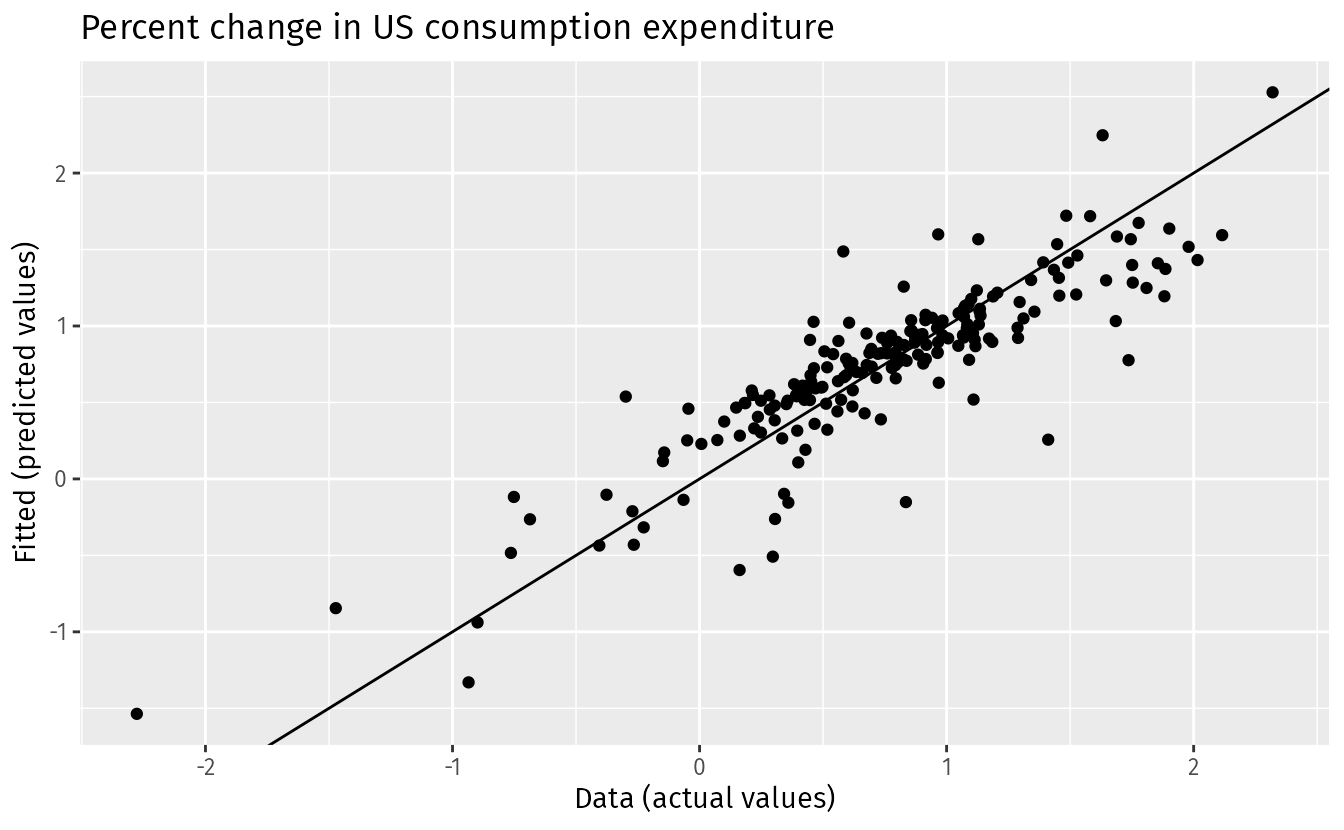
\includegraphics[scale=0.6]{ajustado-vs-real-respuesta.png} 
\end{frame}

\subsection{Bondad de ajuste}
\begin{frame}{Valor de $R^2$}
	\begin{block}{}
		Una forma común de resumir qué tan bien ajusta un modelo de regresión lineal a los datos es calculado el \textbf{coeficiente de determinación:}
		$$ R^2 = \frac{\sum_{t=1}^{T}(y_t - \overline{y})^2}{\sum_{t=1}^{T}(y_t- \hat{y_t})^2} $$
	\end{block}
	
\end{frame}

\begin{frame}{Observaciones del valor de $R^2$}
	\begin{block}{}
		\begin{itemize}
			\item Refleja la \textbf{proporción de la variabilidad} en la variable dependiente $y$ \textbf{que es explicada por el modelo de regresión.}
			\item Validar el rendimiento de pronóstico de un modelo utilizando datos de prueba \textbf{es mucho más confiable que medir} $R^2$ sobre los datos de entrenamiento.
		\end{itemize}
	\end{block}

\end{frame}

\section{Evaluación del modelo de regresión}
\begin{frame}
	\tableofcontents[currentsection] % Solo muestra la sección actual
\end{frame}

\subsection{Sobre los residuos}
\begin{frame}{Definición}
	Las diferencias entre los valores observados de $y$ y los valores ajustados $\hat{y}$ son los \textbf{errores del conjunto de entrenamiento} o \textbf{residuos}, definidos como:
	\begin{block}{Residuos}
		$$ \epsilon_t = y_t - \hat{y_t}$$
	\end{block}

\end{frame}

\begin{frame}{Observaciónes}
	\begin{block}{}
		\begin{itemize}
			\item Es necesario verificar los residuos para asegurarse de que los \textit{supuestos} del modelo se hayan satisfecho.
			\item Se deben realizar una serie de gráficos para evaluar diferentes aspectos de los residuos y del modelo ajustado. 
		\end{itemize}
	\end{block}
\end{frame}

\subsection{Gráficos de residuos}
\begin{frame}{Para evaluar el modelo ajustado}
	\centering
	\begin{block}{}
		\begin{itemize}
			\item Histograma de residuos
			\item Función de autocorrelación de residuos
			\item \textit{Conteo} de residuos
		\end{itemize}
	\end{block}
	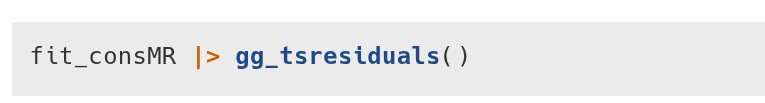
\includegraphics[scale=0.3]{codigo-graficas-residuos.png} 
\end{frame}

\begin{frame}{Para evaluar el modelo ajustado}
	\centering
	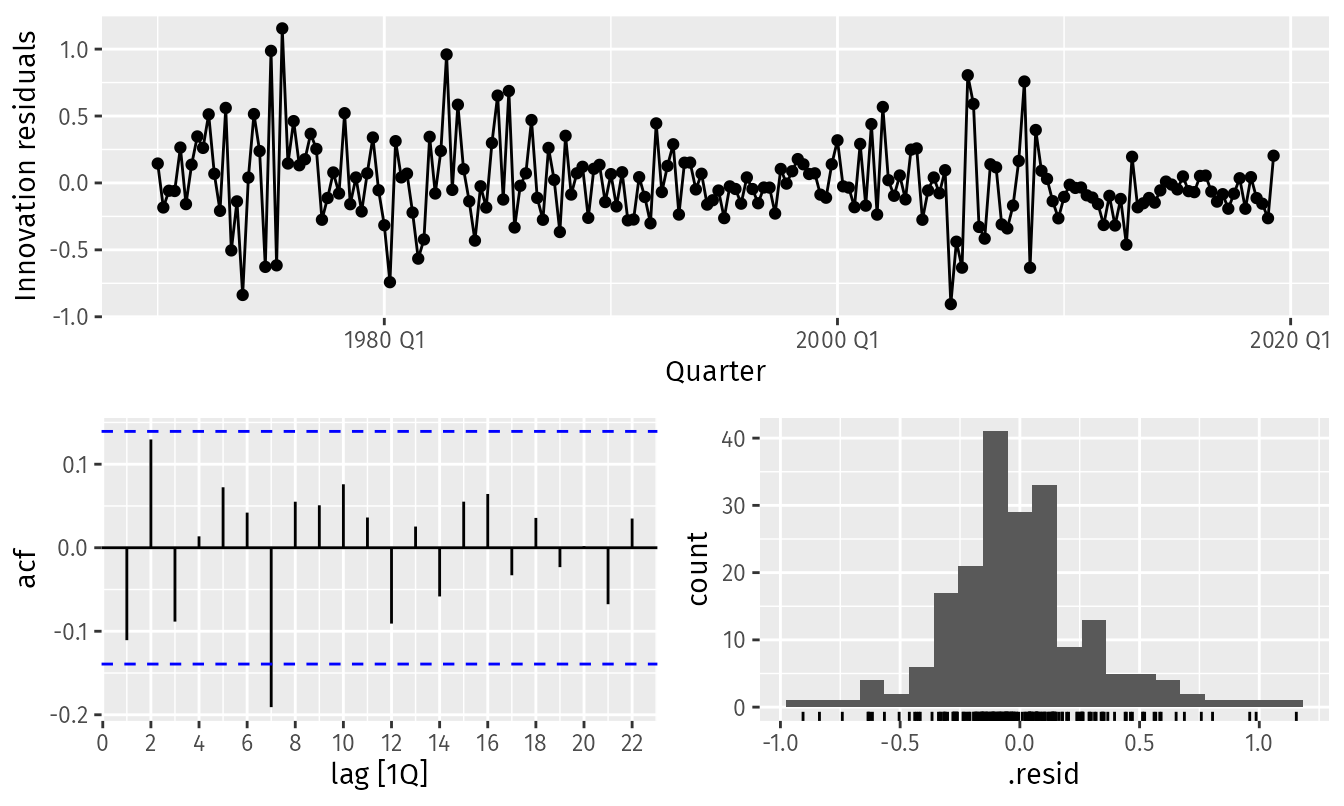
\includegraphics[scale=0.6]{histo-acf-resid.png}
\end{frame}

\begin{frame}{Residuos vs. Predictores}
	\centering
	\begin{block}{}
		 Una forma rápida y sencilla de evaluar el modelo es examinar los \textbf{diagramas de dispersión de los residuos contra cada una de las variables predictoras}. Si estos diagramas muestran un patrón, entonces la relación podría ser no lineal y el modelo necesitaría ser modificado en consecuencia. 
	\end{block}
\end{frame}

\begin{frame}{Residuos vs. Predictores}
	\centering
	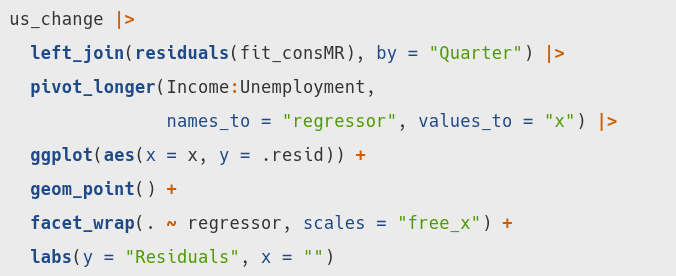
\includegraphics[scale=0.4]{codigo-residuos-predictores.png} 
\end{frame}

\begin{frame}{Residuos vs. Predictores}
	\centering
	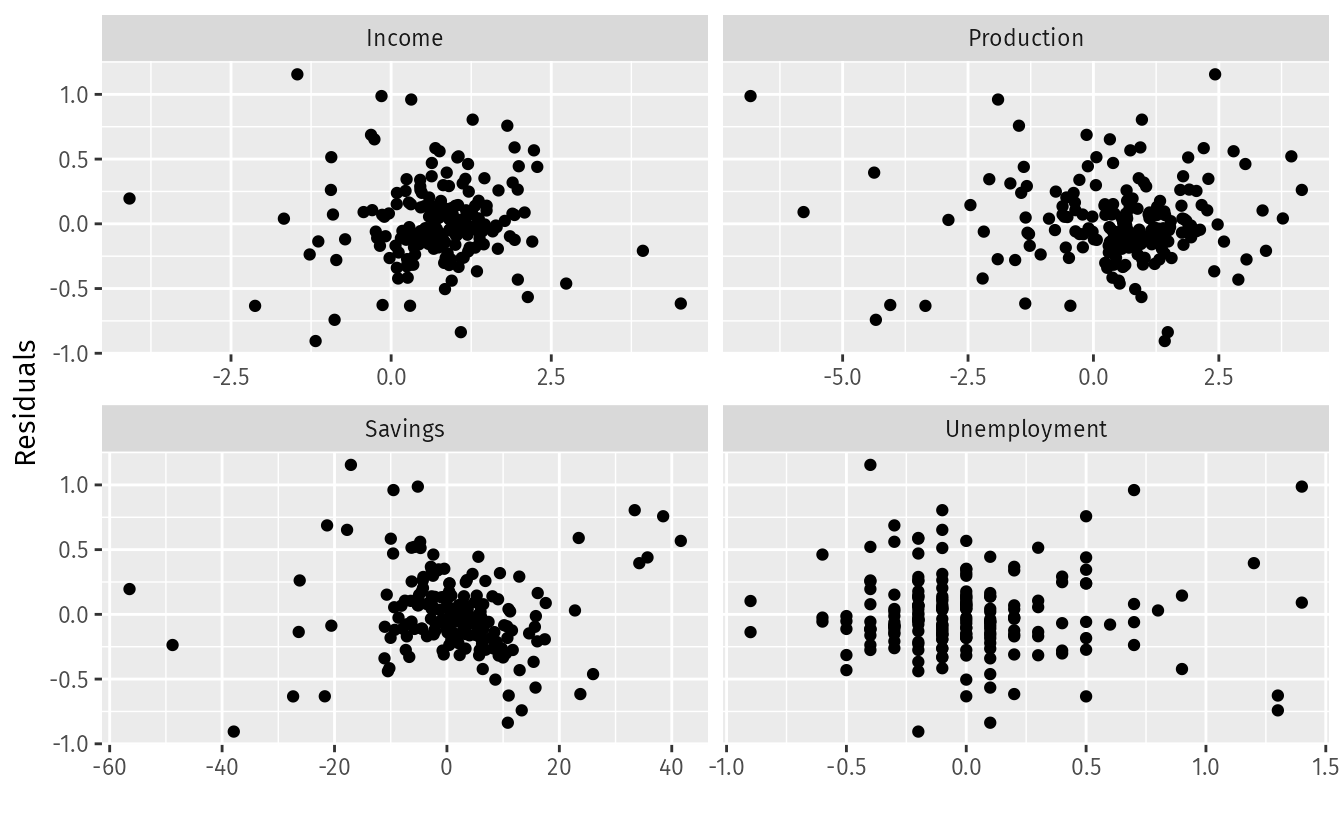
\includegraphics[scale=0.6]{residuos-predictores.png}  
\end{frame}

\begin{frame}{Residuos vs. Valores ajustados}
	\begin{block}{}
		Un gráfico de los residuos contra los valores ajustados también debería mostrar \textbf{ausencia de patrones.}
	\end{block}
	\centering
	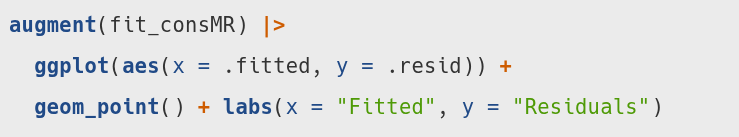
\includegraphics[scale=0.3]{codigo-residuos-ajutados.png} 
\end{frame}

\begin{frame}{Residuos vs. Valores ajustados}
	\centering
	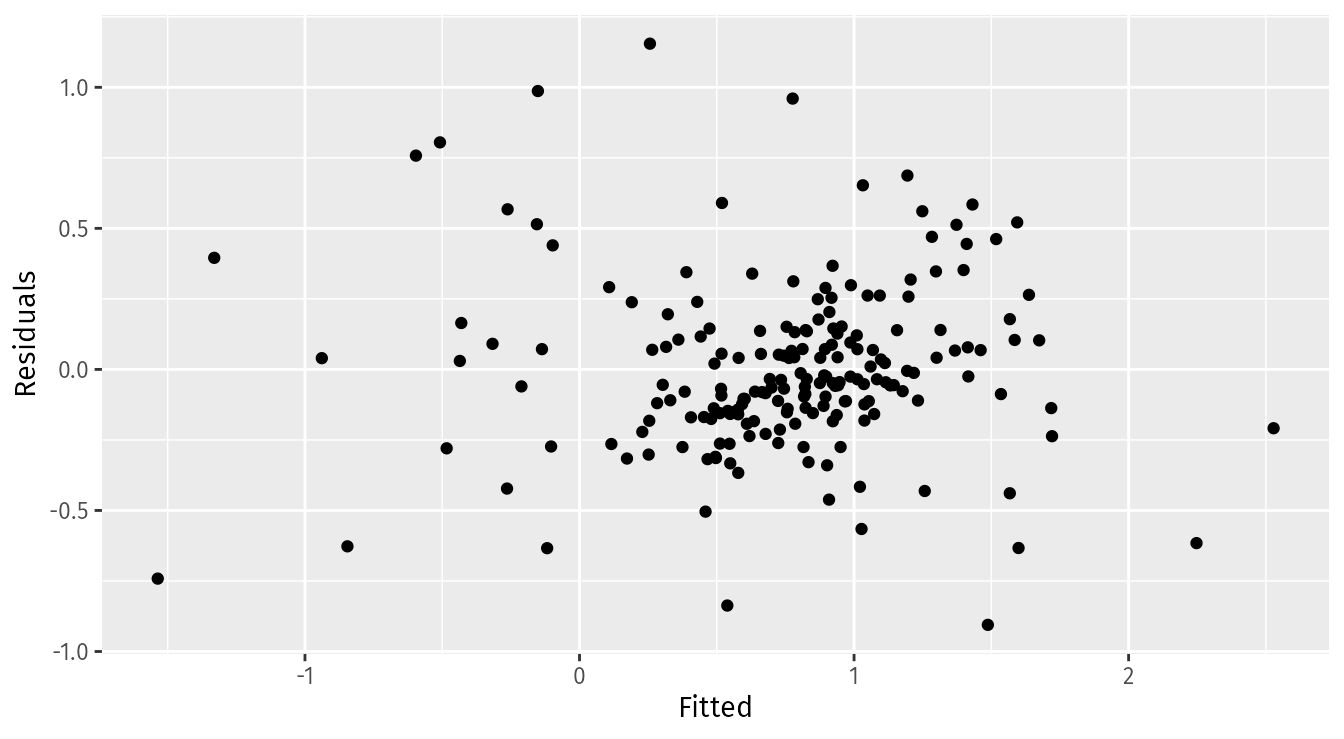
\includegraphics[scale=0.6]{residuos-ajutados.png} 
\end{frame}

\section{Predictores útiles}
\begin{frame}
	\tableofcontents[currentsection] % Solo muestra la sección actual
\end{frame}
\subsection{Tendencia (Trend)}
\begin{frame}{Definición}
	\vspace{-1cm}
	\begin{block}{}
		Es común que los datos de series de tiempo muestren tendencia. Una tendencia lineal puede modelarse utilizando simplemente $x_{1,t} = t$ como un predictor, con el modelo de regresión:
		$$ y_t= \beta_0 + \beta_1 t + \epsilon_t  $$
		Una variable de tendencia puede ser especificada en la función \textbf{TSLM()} usando el comando especial \textbf{trend().}
	\end{block}
\end{frame}

\subsection{Variables dummy}
\begin{frame}{Definición}
	\begin{block}{}
		Cuando un predictor es una \textbf{variable categórica} que toma solo dos valores, se puede manejar creando una \textit{variable dummy} que:
		\begin{itemize}
			\item Toma el valor $1$ correspondiente a \textit{sí}
			\item Toma el valor $0$ correspondiente a \textit{no}
		\end{itemize}				
		Una \textit{variable dummy} también es conocida como \textit{variable indicadora}.
	\end{block}
\end{frame}

\begin{frame}{Ejemplo de uso}
	\begin{block}{}
	\begin{table}[h!]
		\centering
		\begin{tabular}{|c|c|c|c|c|c|c|}
			\hline
			Día & $d_{1,t}$ & $d_{2,t}$ & $d_{3,t}$ & $d_{4,t}$ & $d_{5,t}$ & $d_{6,t}$ \\
			\hline
			Lunes & 1 & 0 & 0 & 0 & 0 & 0 \\
			Martes & 0 & 1 & 0 & 0 & 0 & 0 \\
			Miércoles & 0 & 0 & 1 & 0 & 0 & 0 \\
			Jueves & 0 & 0 & 0 & 1 & 0 & 0 \\
			Viernes & 0 & 0 & 0 & 0 & 1 & 0 \\
			Sábado & 0 & 0 & 0 & 0 & 0 & 1 \\
			Domingo & 0 & 0 & 0 & 0 & 0 & 0 \\
			\hline
		\end{tabular}
		\caption{Tabla de variables dummy para días de la semana}
	\end{table}
	\end{block}
\end{frame}

\begin{frame}{Trampa de la variable dummy}
	\begin{block}{}
		Se le conoce como \textbf{\textit{trampa de la variable dummy}} a la situación en la que se incluye una variable dummy adicional para una categoría extra, lo que \textit{genera un exceso de parámetros por estimar. }
	\end{block}
	
	\begin{block}{Regla general}
		Usar \textbf{una variable dummy menos que el número de categorías.} Por ejemplo, con datos semanales, se deben usar seis variables dummy.
	\end{block}
\end{frame}

\subsection{Aplicación}
\begin{frame}{Ejemplo de producción trimestral de cerveza en Australia}
	\vspace{-1cm}
	\begin{block}{}
		La base de datos utilizada en este ejemplo contiene registros históricos de la producción de cerveza en Australia, desglosados por trimestre. Los datos incluyen:
		\begin{itemize}
			\item \textbf{Fecha}: Cada registro corresponde a un trimestre específico.
			\item \textbf{Cantidad de cerveza producida:} Medida en megalitros, que es una unidad de volumen que equivale a un millón de litros.
		\end{itemize}
	\end{block}
\end{frame}

\begin{frame}{Ejemplo de producción trimestral de cerveza en Australia}
	\centering
	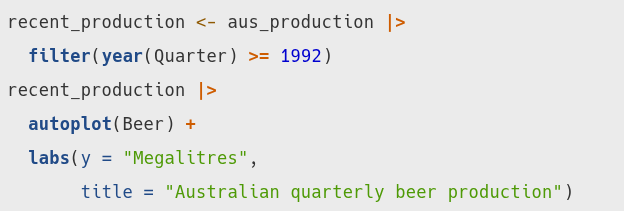
\includegraphics[scale=0.5]{codigo-australia-cerveza.png} 
\end{frame}

\begin{frame}{Ejemplo de producción trimestral de cerveza en Australia}
	\centering
	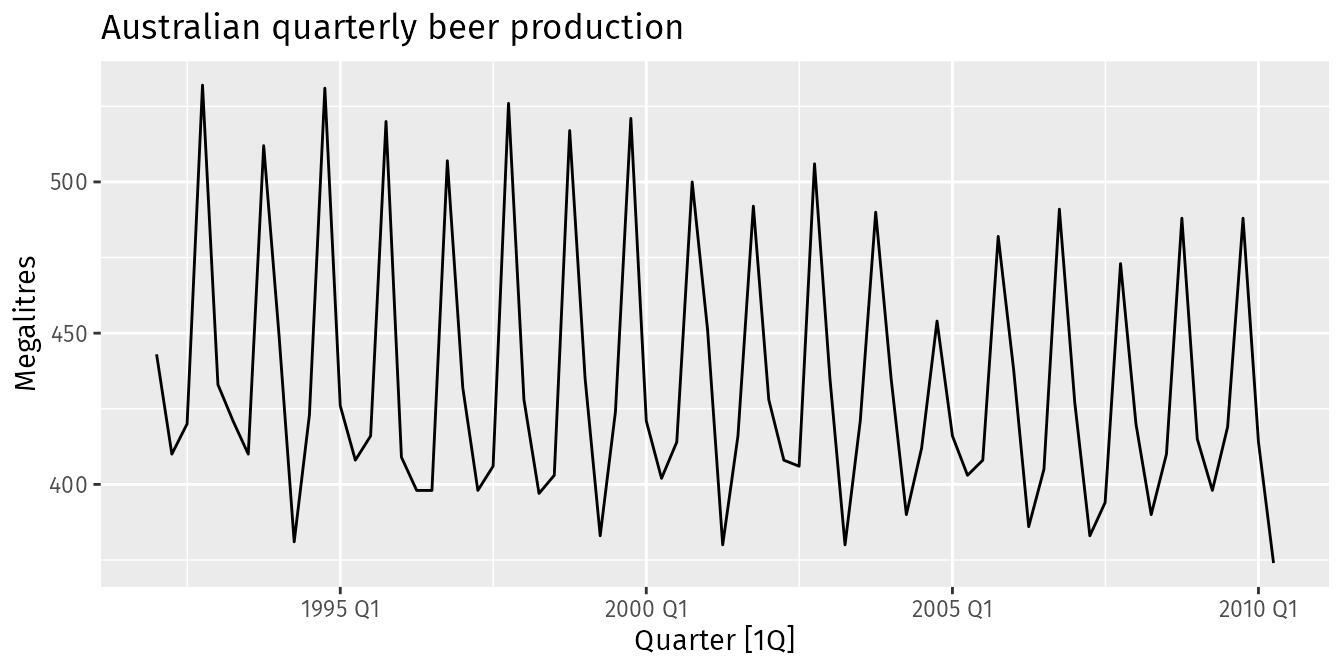
\includegraphics[scale=0.6]{-1.png} 
\end{frame}

\begin{frame}{Ejemplo de producción trimestral de cerveza en Australia}
	\begin{block}{}
		Queremos pronosticar el valor de la \textbf{producción futura de cerveza.} Podemos modelar estos datos utilizando un \textit{modelo de regresión con una tendencia lineal y variables dummy trimestrales:}
		$$ y_t = \beta_0+\beta_1t+\beta_2 d_{2,t} + \beta_3 d_{3,t} + \beta_4 d_{4,t} + \epsilon_t$$
	\end{block}
\end{frame}

\begin{frame}{Ejemplo de producción trimestral de cerveza en Australia}
	\centering
	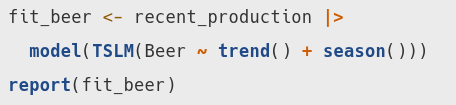
\includegraphics[scale=0.5]{codigo-modelo-cerveza.png} 
\end{frame}

\begin{frame}{Ejemplo de producción trimestral de cerveza en Australia}
	\centering
	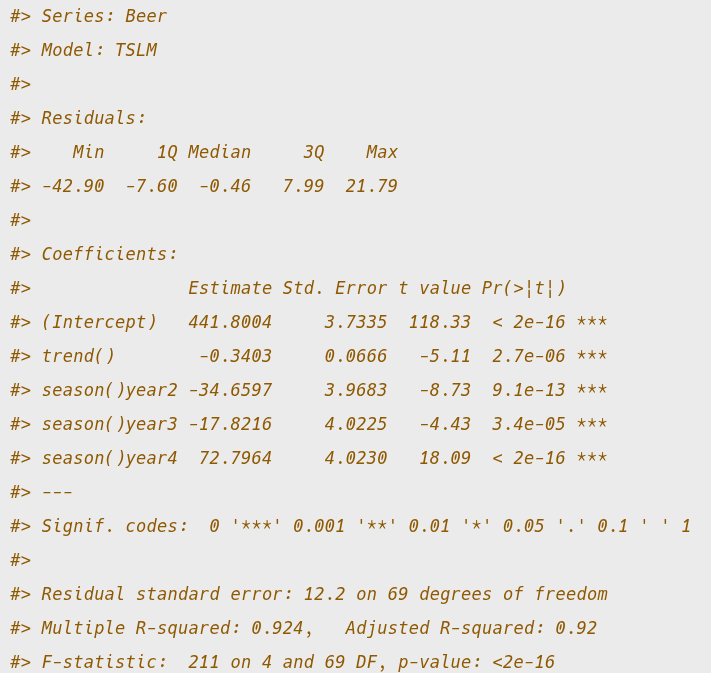
\includegraphics[scale=0.3]{reporte-modelo-cerveza.png} 
\end{frame}

\begin{frame}{Ejemplo de producción trimestral de cerveza en Australia}
	\begin{block}{}
		\begin{itemize}
			\item \textbf{Tendencia 1:} Existe una tendencia descendente promedio de -0.34 megalitros por trimestre.
			\item \textbf{Trimestre 2:} En promedio, la producción es 34.7 megalitros menor que en el primer trimestre.
			\item \textbf{Trimestre 3:} En promedio, la producción es 17.8 megalitros menor que en el primer trimestre.
			\item \textbf{Trimestre 4:} En promedio, la producción es 72.8 megalitros mayor que en el primer trimestre.
		\end{itemize}
	\end{block}
\end{frame}

\begin{frame}{Modelo ajustado y Real}
	\centering
	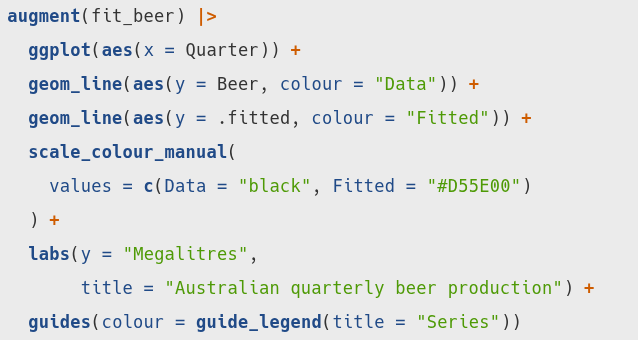
\includegraphics[scale=0.5]{codigo-ajustado-y-real.png} 
\end{frame}

\begin{frame}{Modelo ajustado y Real}
	\centering
	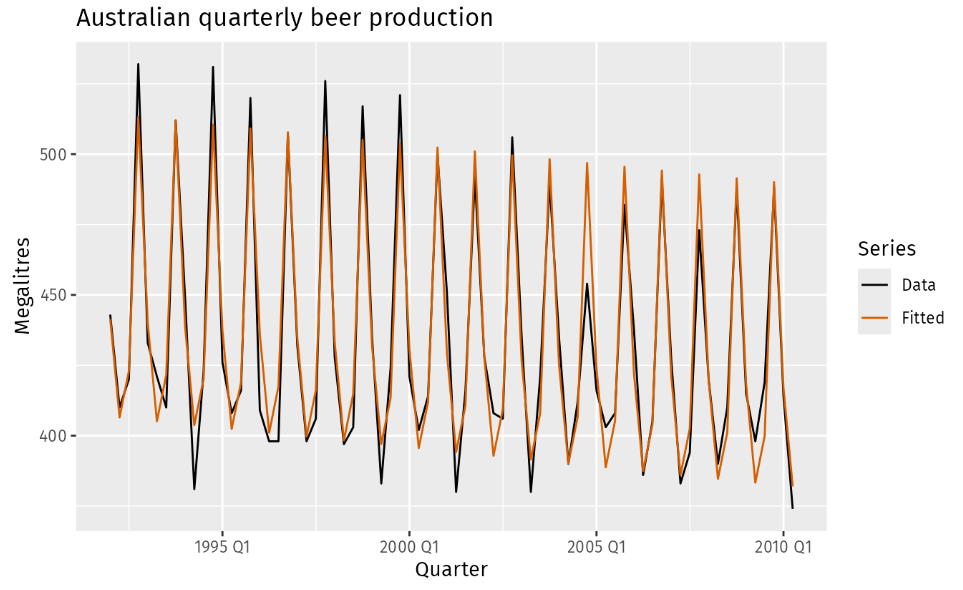
\includegraphics[scale=0.3]{ajustado-y-real-cerveza.png} 
\end{frame}

\begin{frame}{Modelo ajustado vs. Real}
	\centering
	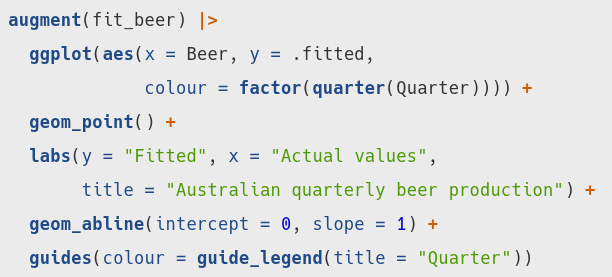
\includegraphics[scale=0.3]{cerverza-colores1.png} 
\end{frame}

\begin{frame}{Modelo ajustado vs. Real}
	\centering
	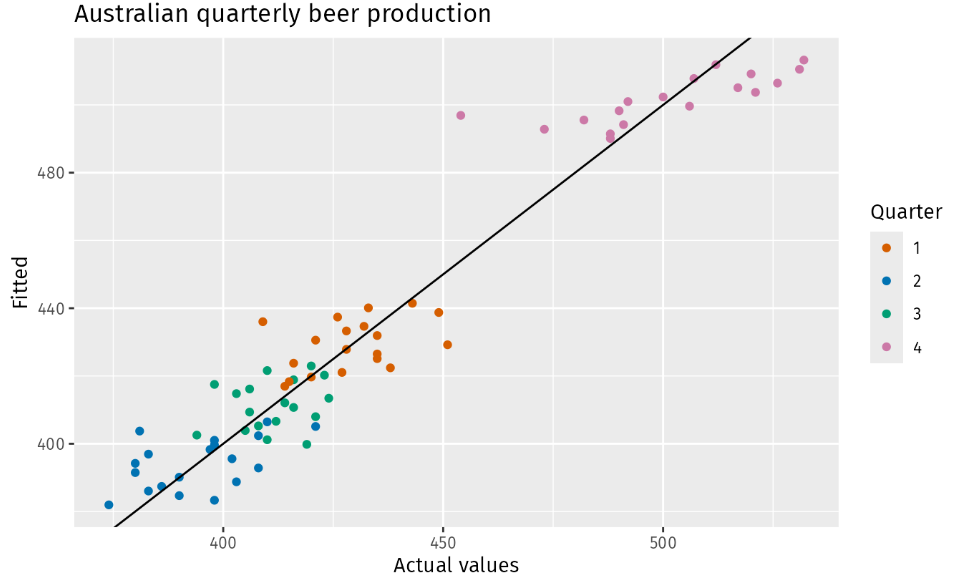
\includegraphics[scale=0.3]{cerverza-colores2.png} 
\end{frame}

\section{Variables de intervención}
\begin{frame}
	\tableofcontents[currentsection] % Solo muestra la sección actual
\end{frame}

\begin{frame}{Modelar intervenciones}
	\begin{block}{}
		A menudo es necesario modelar intervenciones que pueden haber afectado la variable que estamos pronosticando. Por ejemplo:
		\begin{itemize}
			\item Actividades de competidores
			\item Gastos en publicidad
			\item Medidas laborales
		\end{itemize}
		entre otros, pueden tener un impacto significativo en los datos.
	\end{block}
\end{frame}

\subsection{Variables \textit{spike}}
\begin{frame}{Modelar intervenciones}
	\begin{block}{}
		Cuando el efecto de la intervención dura solo un periodo, se utiliza una variable \textit{spike}. Esta es una variable \textit{dummy} que toma el valor de $1$ en el \textbf{periodo de la intervención} y $0$ en \textbf{los demás periodos}.
		\begin{itemize}
			\item \textbf{Ejemplo}: Si una campaña publicitaria ocurre durante un trimestre específico, la variable \textit{spike} será 1 solo para ese trimestre y 0 para los demás.
		\end{itemize}
	\end{block}
\end{frame}

\begin{frame}{Modelar intervenciones}
	\begin{block}{}
		Cuando el efecto de la intervención dura solo un periodo, se utiliza una variable \textit{spike}. Esta es una variable \textit{dummy} que toma el valor de $1$ en el \textbf{periodo de la intervención} y $0$ en \textbf{los demás periodos}.
		\begin{itemize}
			\item \textbf{Ejemplo}: Si una campaña publicitaria ocurre durante un trimestre específico, la variable \textit{spike} será 1 solo para ese trimestre y 0 para los demás.
		\end{itemize}
	\end{block}
	\begin{block}{Equivalencia}
		Una variable \textit{spike} es equivalente a una variable dummy para manejar un valor atípico.
	\end{block}
\end{frame}

\subsection{Variables \textit{step}}
\begin{frame}{Modelar intervenciones}
	\begin{block}{}
		Si una intervención provoca un \textbf{cambio de nivel} (es decir, el valor de la serie cambia de manera repentina y permanente desde el momento de la intervención), entonces utilizamos una variable \textit{step}.
		\begin{itemize}
			\item Toma el valor de 0 antes de la intervención.
			\item Toma el valor de 1 después de la intervención\footnote{lo que indica que el efecto se mantiene de manera \textbf{permanente}.} 
		\end{itemize}
	\end{block}
\end{frame}

\subsection{Cambio en la pendiente}
\begin{frame}{Modelar intervenciones}
	\begin{block}{}
		Un tipo de \textbf{efecto permanente} es un cambio en la pendiente de la serie. En este caso, la intervención se maneja mediante una tendencia lineal a tramos \textit{(piecewise linear trend)}, lo que significa que la tendencia cambia en el momento de la intervención y se vuelve no lineal.
			\begin{itemize}{}
				\item \textbf{Características}: La tendencia se ajusta a una nueva pendiente a partir del momento de la intervención.
			\end{itemize}
	\end{block}
\end{frame}

\section*{Gracias}
\begin{frame}
	\tableofcontents[currentsection] % Solo muestra la sección actual
\end{frame}
\begin{frame}{Por su atención}
	\centering
	\Huge
	\titulaso{Gracias.}
\end{frame}


\end{document}